\documentclass[letterpaper,11pt]{article}

\usepackage[open,openlevel=1]{bookmark}
\usepackage{amsmath}
\usepackage{graphicx}
\usepackage[ruled,vlined]{algorithm2e}
\usepackage{mcode}
\usepackage{subcaption}

% The percent sign indicates comments and does not effect what is written to the pdf

% If you would like to include figures use

% For inline equations, enclose with dollar signs ex. $\frac{1}{2}$

% For equation blocks use \begin{align} ... \end{align} for numbered equations and \begin{align*} \end{align*} for non numbered equations

% To include a figure, you can use the following command, or use it as a template
% To use this command type "\Figure{filename.png}{figure caption}{figure label}

\newcommand{\Figure}[3]{
%\Figure{File}{Caption}{Reference}
\begin{figure}[h]
\begin{center}
\includegraphics[width=3.5in]{#1}
\caption{#2}
\label{fig:#3}
\end{center}
\end{figure}
}

%%%%%%%%%%%%%%%%%%%%%%%%%%%%%%%%%%%%%%%%%%%%%%%%%%%%%%
%%%%%%%%%%%%%%%%% End of Preamble %%%%%%%%%%%%%%%%%%%%
%%%%%%%%%%%%%%%%%%%%%%%%%%%%%%%%%%%%%%%%%%%%%%%%%%%%%%

%%%%%%%%%%%%%%%%%%%%%%%%%%%%%%%%%%%%%%%%%%%%%%%%%%%%%%
%%%%%%%%%%% Document content start here %%%%%%%%%%%%%%
%%%%%%%%%%%%%%%%%%%%%%%%%%%%%%%%%%%%%%%%%%%%%%%%%%%%%%

\begin{document}

\title{Project 1: Fractal Geometry \\ 
		\large MAT128B Winter 2020}
\author{Caitlin Brown, Nikos Trembois, and Shuai Zhi}
\date{February 19, 2020}
\maketitle
\tableofcontents
\newpage

\section{Introduction}
In this project, numerical analysis is used to understand and demonstrate fractals and their characteristics. The fractals will be generated from the orbits of complex functions. Orbits are the sequence of numbers that results from the process of applying a function to the output of the same function over and over, like a recursive function. So $orb(z_0) = z_0, z_1 = \phi(z_0), z_2 \phi(\phi(z_0)) ...$ is the orbit of the initial point $z_0$ under the function $\phi$. It is not hard to imagine that for certain initial values this process will diverge while other initial values will converge, or at least remain bounded by some value. The filled Julia set is all points whose orbit, using a polynomial function, remains bounded. The boundary of the filled set is called the Julia set.

\section{Unit Disk}
The orbit of complex values whose real and imaginary part were within [-1, 1] were calculated for the function $\phi(z) = z^2$. The filled Julia set of $\phi(z) = z^2$, shown in figure \ref{fig:unitDisk}, shows the map the orbit, which is the unit disk. Under the same conditions the Julia set would create the unit circle, as it is the boundary of the filled Julia set. 

\begin{figure}
	\centering
	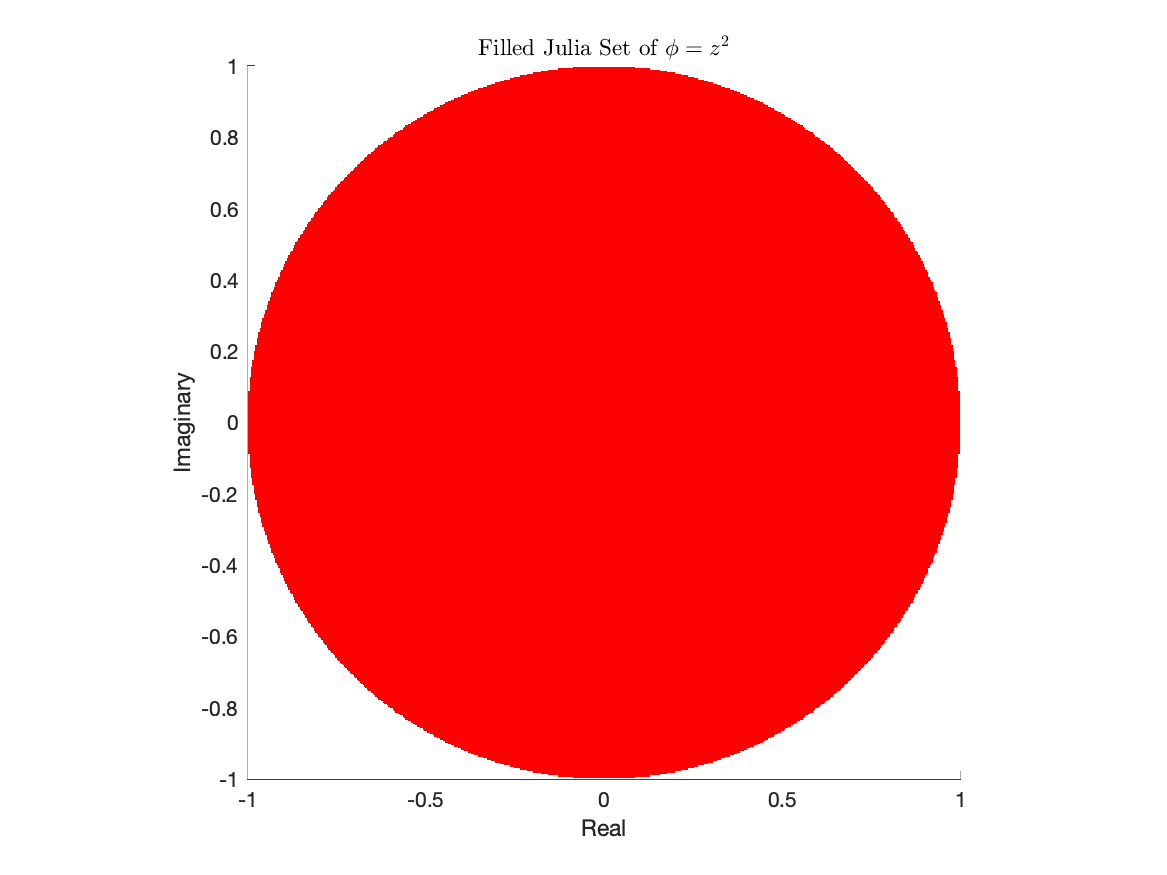
\includegraphics[width=3.5in]{../Figures/UnitDisk.png}
	\caption{Orbit of $z = a + bi$ for $a = b = [-1,1]$ under $\phi=z^2$}
	\label{fig:unitDisk}
\end{figure}

\section{Introduction to Fractals}
The unit disk is a great illustration of the orbit of different initial points under $\phi=z^2$. However, adding a constant to the function (i.e. $\phi(z) = z^2 + c$) creates more interesting maps, which turn out to be fractals. 

\begin{figure}
\centering
	\begin{subfigure}[b]{0.49\linewidth}
		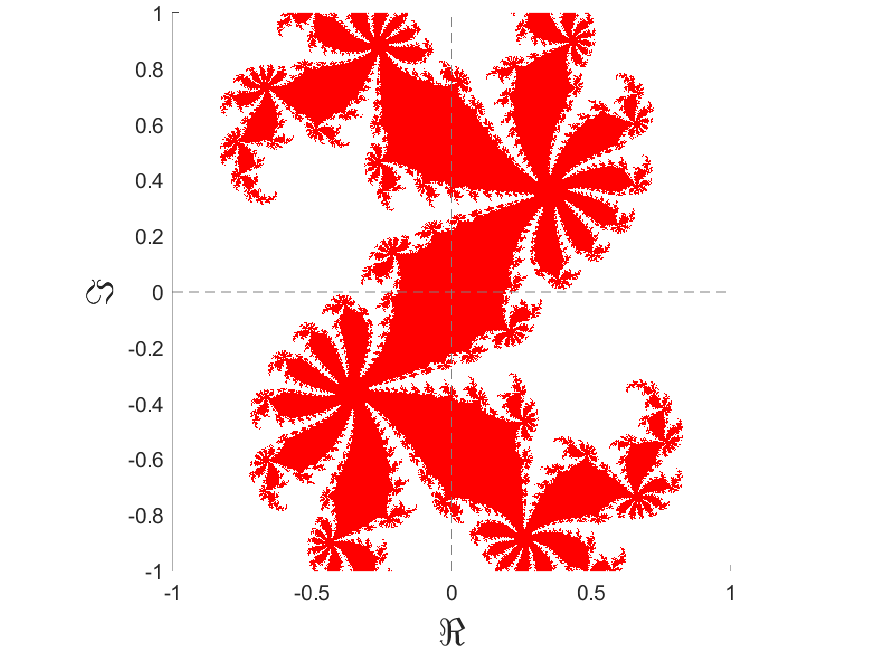
\includegraphics[width=\linewidth]{../Figures/FilledJulia1.png}
		\caption{Filled Julia Set of $z = 0.36 + 0.1i$}
		\label{fig:FJ+.36+.1i}
	\end{subfigure}
	\begin{subfigure}[b]{0.49\linewidth}
		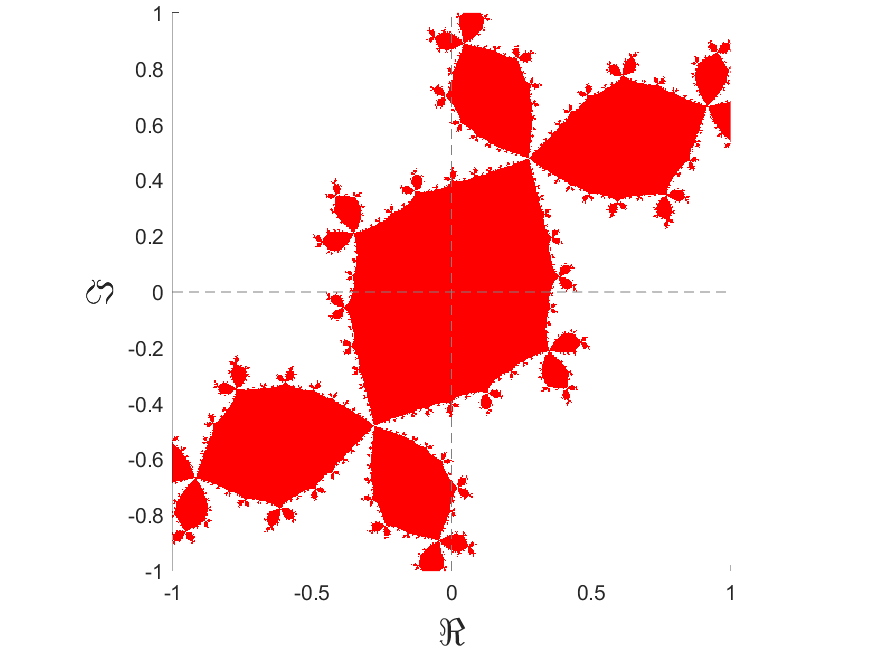
\includegraphics[width=\linewidth]{../Figures/FilledJulia2.png}
		\caption{Filled Julia Set of $z = -0.123 + 0.745i$}
		\label{fig:FJ+.123+.745i}
	\end{subfigure}
	
	\vskip\baselineskip
	
	\begin{subfigure}[b]{0.49\textwidth}
		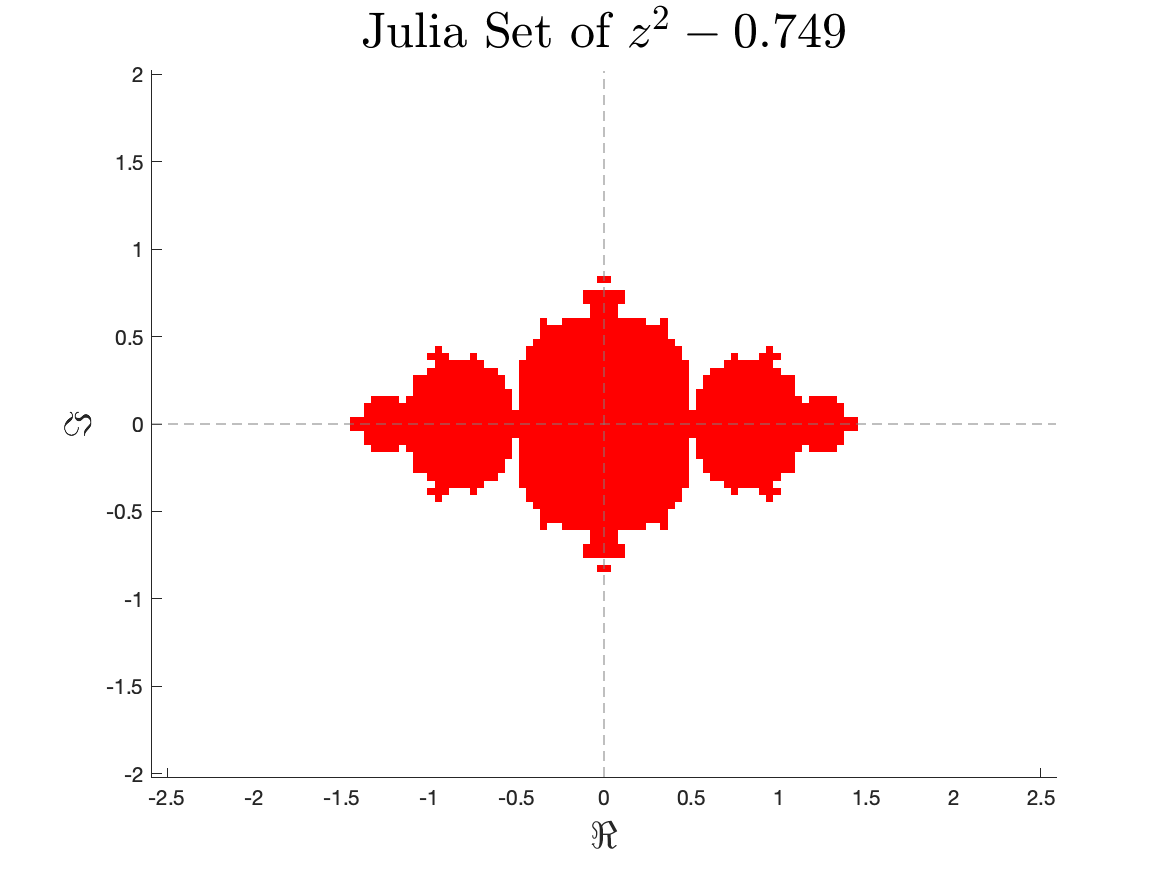
\includegraphics[width=\textwidth]{../Figures/FilledJulia3.png}
		\caption{Filled Julia Set of $z = - 0.749$}
		\label{fig:FJ-.749}
	\end{subfigure}
	\begin{subfigure}[b]{0.49\textwidth}
		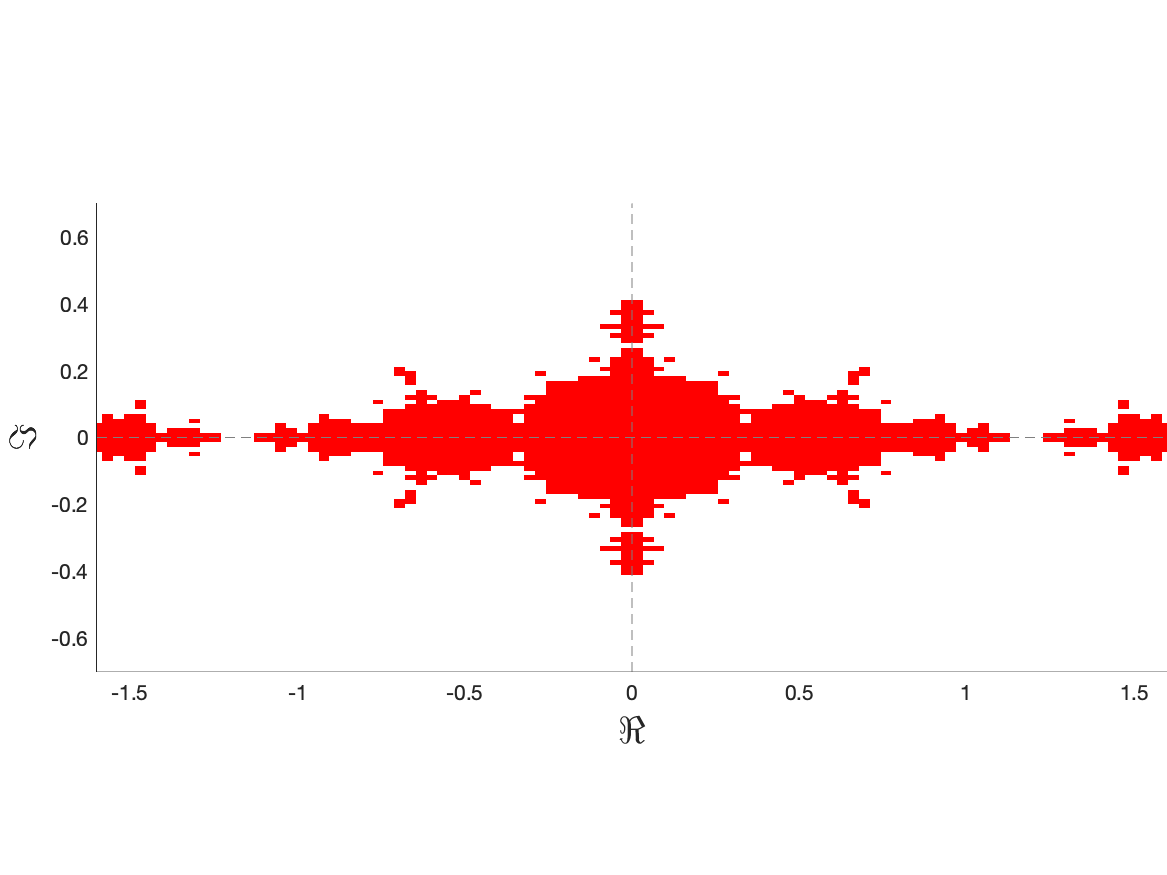
\includegraphics[width=\textwidth]{../Figures/FilledJulia4.png}
		\caption{Filled Julia Set of $z = -1.25$}
		\label{fig:FJ-1.25}
	\end{subfigure}
	\caption{Filled Julia sets with 100 points in real and imaginary axis}
	\label{fig:FJwithC}
\end{figure}

\section{Julia Set}
The Julia set shows is the boundary of the filled Julia set. So, it marks the edge of the points whose orbits converge under a given function. All points inside the outline converge, including the line, while those outside of it diverge. The Julia set is found using the inverse iteration method, which is an attractor. 

\begin{figure}
\centering
	\begin{subfigure}[b]{0.49\linewidth}
		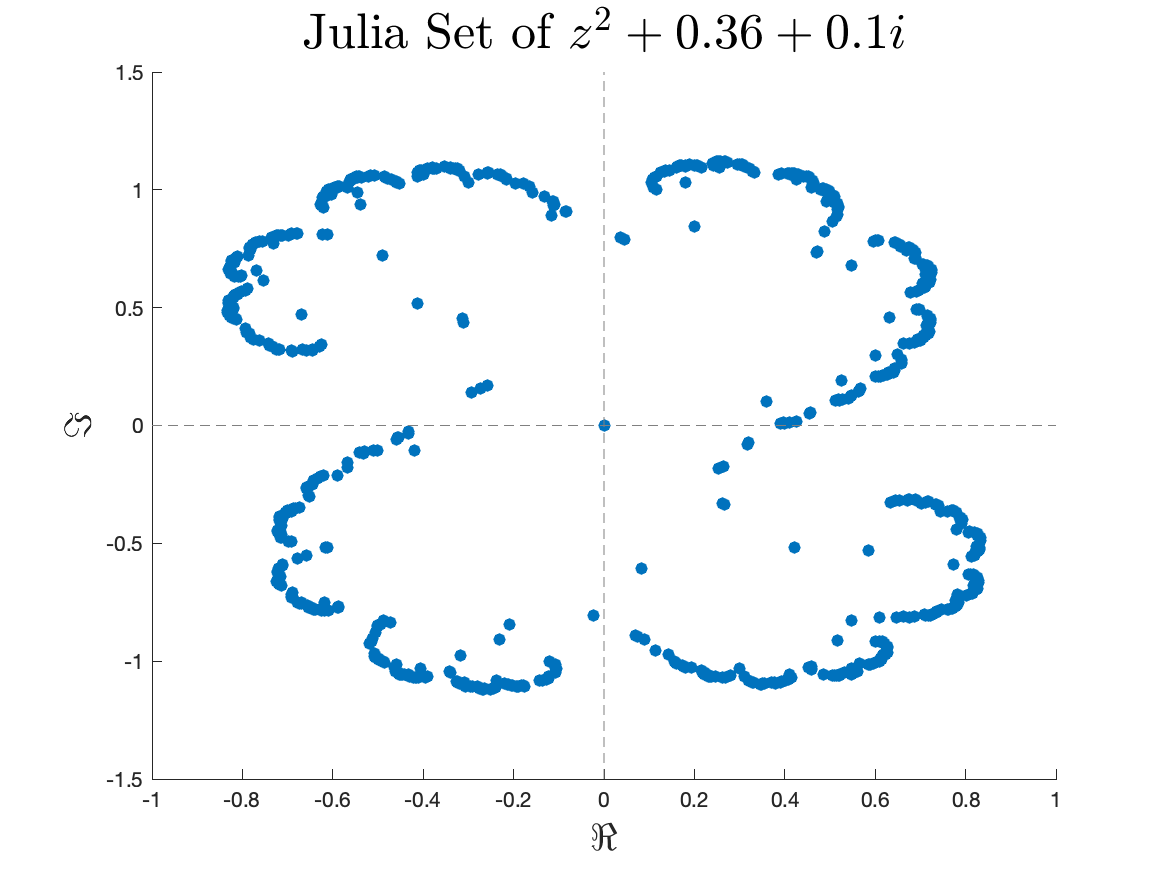
\includegraphics[width=\linewidth]{../Figures/Julia1.png}
		\caption{Julia Set of $z = 0.36 + 0.1i$}
		\label{fig:J+.36+.1i}
	\end{subfigure}
	\begin{subfigure}[b]{0.49\linewidth}
		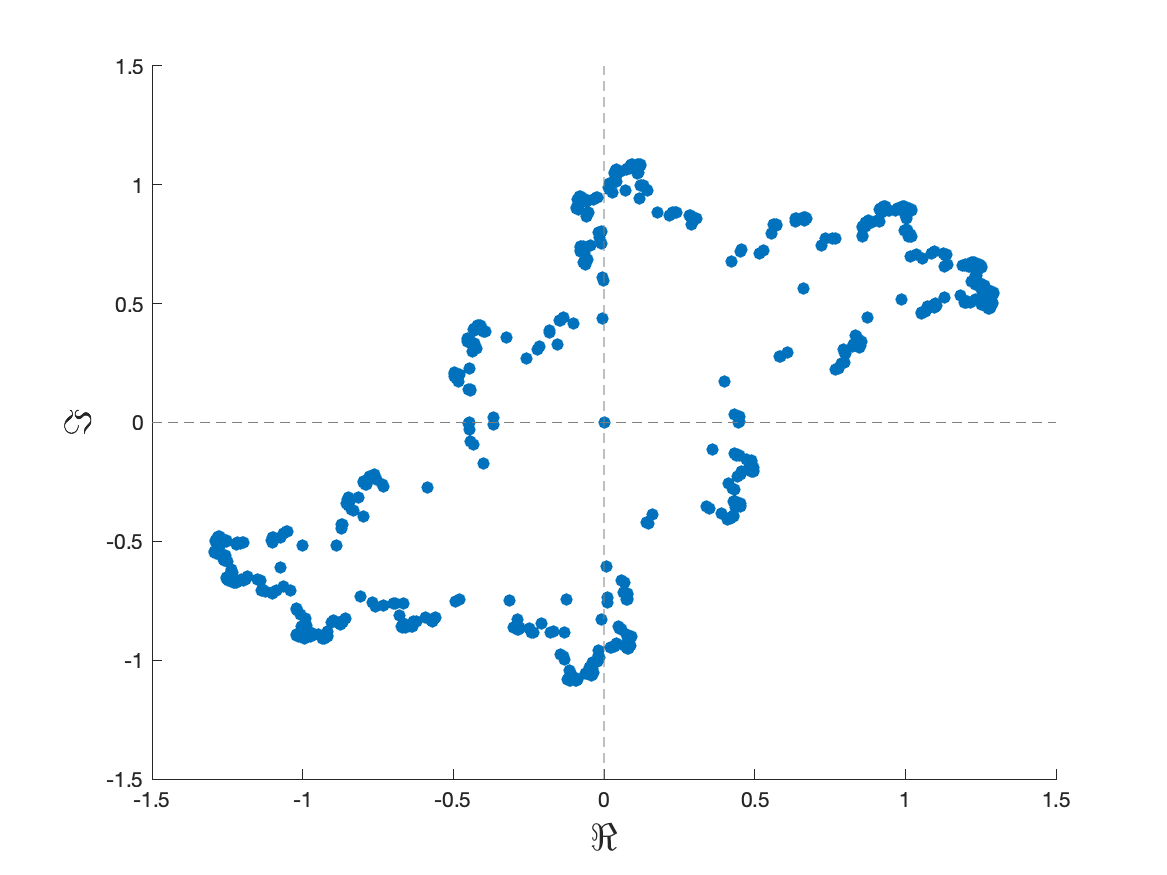
\includegraphics[width=\linewidth]{../Figures/Julia2.png}
		\caption{Julia Set of $z = -0.123 + 0.745i$}
		\label{fig:J+.123+.745i}
	\end{subfigure}
	
	\vskip\baselineskip
	
	\begin{subfigure}[b]{0.49\textwidth}
		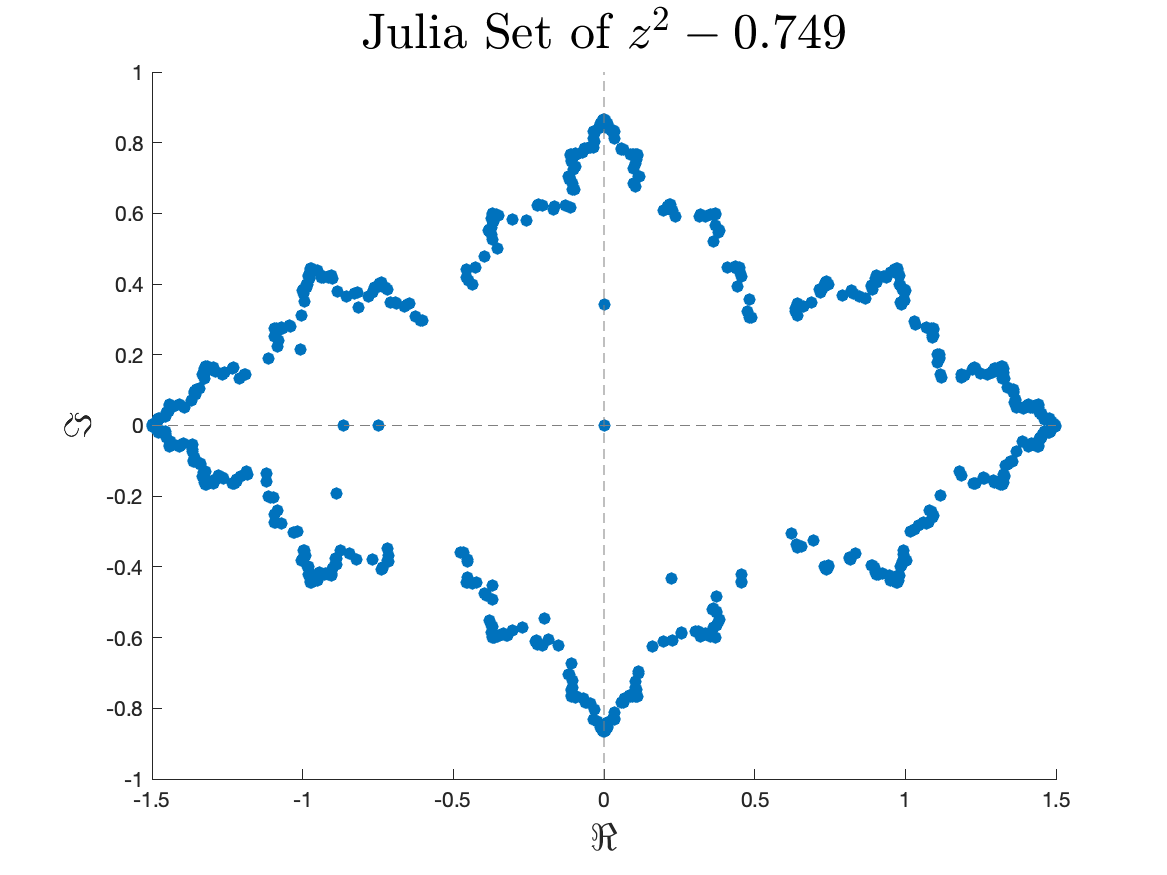
\includegraphics[width=\textwidth]{../Figures/Julia3.png}
		\caption{Julia Set of $z = - 0.749$}
		\label{fig:J-.749}
	\end{subfigure}
	\begin{subfigure}[b]{0.49\textwidth}
		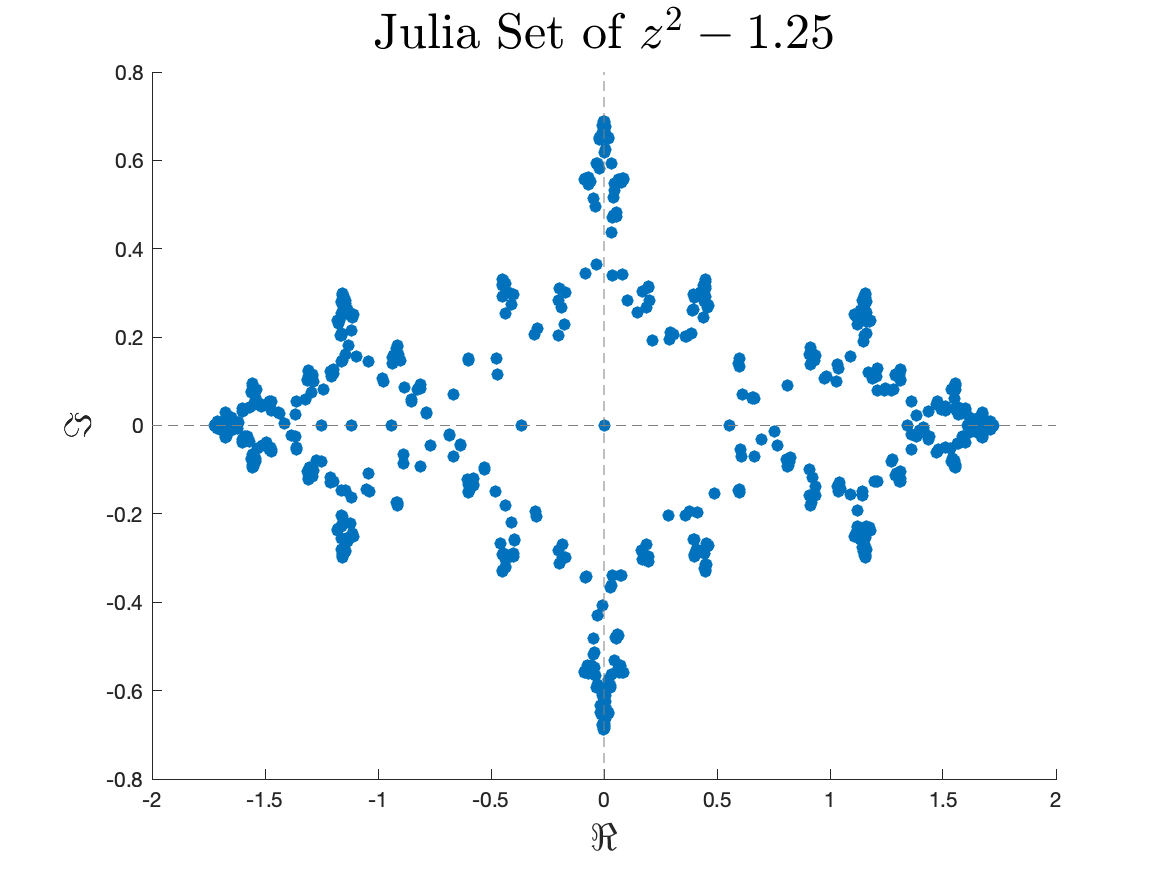
\includegraphics[width=\textwidth]{../Figures/Julia4.png}
		\caption{Julia Set of $z = -1.25$}
		\label{fig:J-1.25}
	\end{subfigure}
	\caption{Julia sets with 10,000 iterations of the inverse function}
	\label{fig:Julia}
\end{figure}

\section{Fractal Dimensions}

\section{Julia Set Connectivity}
A Julia set is considered connected if a point in the set can travel to another point in the set without having to leave the set. In other words, there is only one boundary that encloses all points. Julia discovered a simple criterion to determine if Julia sets are connected. He found that if the orbit of the initial point 0 is bounded, then the set is connected, otherwise it is not. Therefore, the connectivity of set under the function $\phi(z)$ can be easily found, but careful consideration must be required for number of iterations to use. Too few iterations may not be enough to capture the diverging effect of the orbit, while to many may require an unnecessary number of computations.

\section{Divergent Orbits}
The number of iterations it takes for a value to diverge creates interesting plots where it is 

\begin{figure}
\centering
	\begin{subfigure}[b]{0.49\linewidth}
		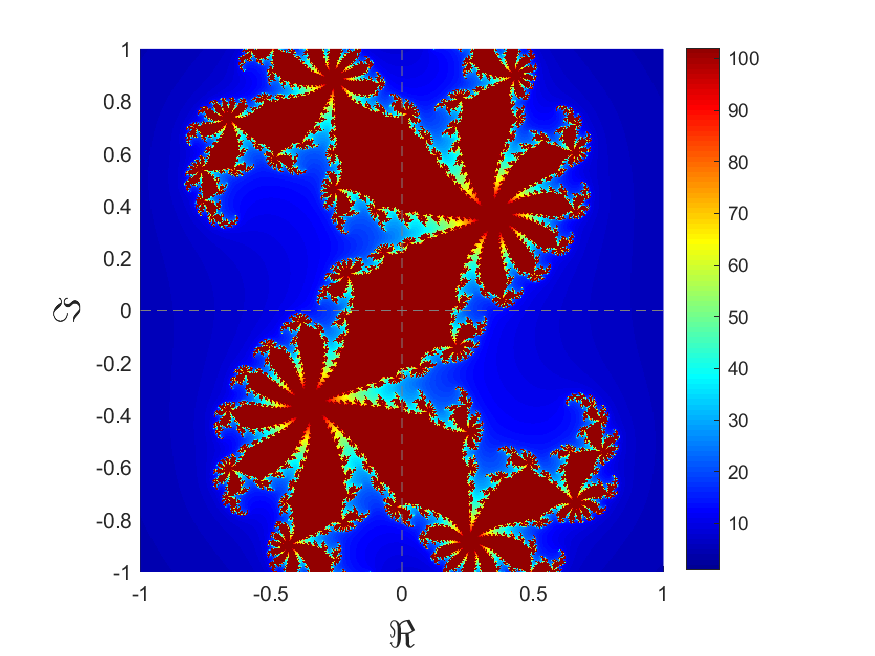
\includegraphics[width=\linewidth]{../Figures/ColoredJulia1.png}
		\caption{Julia Set of $z = 0.36 + 0.1i$}
		\label{fig:CJ+.36+.1i}
	\end{subfigure}
	\begin{subfigure}[b]{0.49\linewidth}
		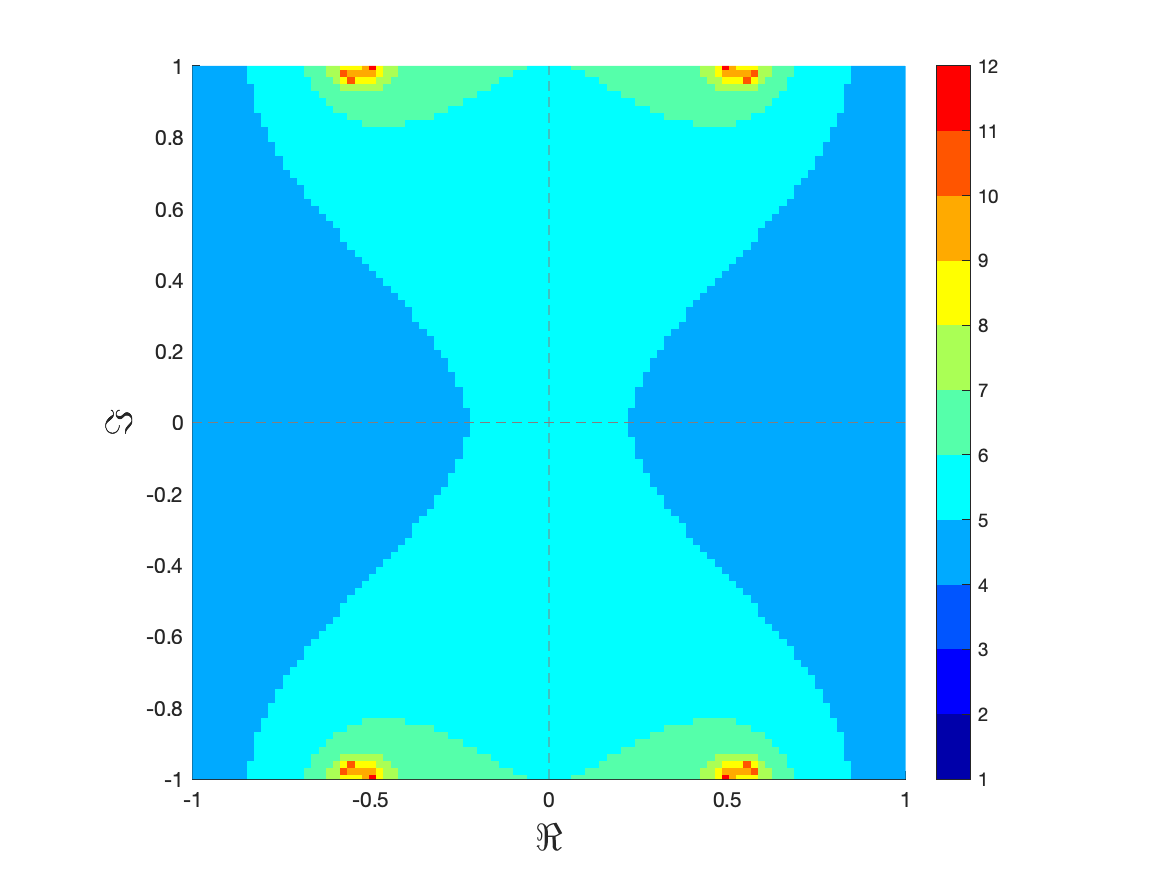
\includegraphics[width=\linewidth]{../Figures/ColoredJulia2.png}
		\caption{Julia Set of $z = -0.123 + 0.745i$}
		\label{fig:CJ+.123+.745i}
	\end{subfigure}
	
	\vskip\baselineskip
	
	\begin{subfigure}[b]{0.49\textwidth}
		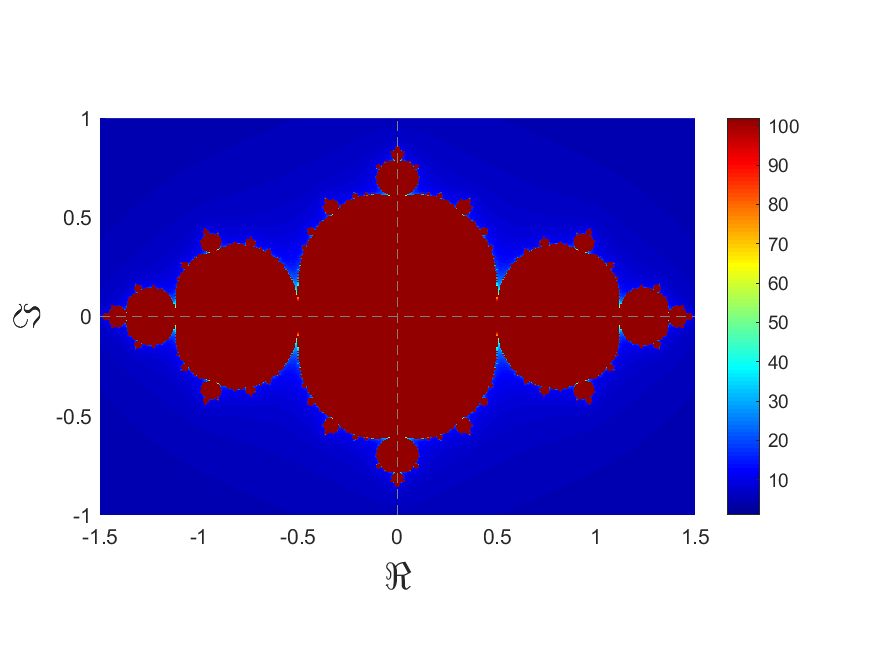
\includegraphics[width=\textwidth]{../Figures/ColoredJulia3.png}
		\caption{Julia Set of $z = - 0.749$}
		\label{fig:CJ-.749}
	\end{subfigure}
	\begin{subfigure}[b]{0.49\textwidth}
		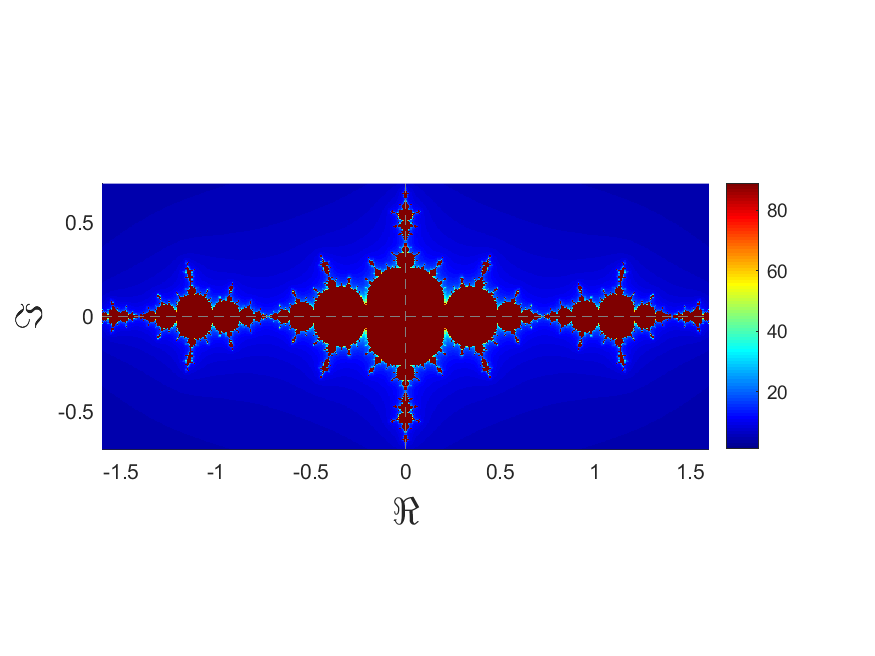
\includegraphics[width=\textwidth]{../Figures/ColoredJulia4.png}
		\caption{Julia Set of $z = -1.25$}
		\label{fig:CJ-1.25}
	\end{subfigure}
	\caption{Filled Julia sets colored based on number of iterations to converge}
	\label{fig:FJwithC}
\end{figure}

\section{Newton's Method in Complex Plane}
Root finding can be a surprisingly difficult task. The linear case is trivial and roots of second order polynomials are solved with the quadratic equation. However, as the order increases the analytic equations to solve for the roots become more intricate and no known analytic equation exists for polynomials of orders higher than 6. Not to mention, this is just for real functions! Finding the roots of complex functions is even more difficult. Fortunately iterative methods, with the help of plots, simplify the process; although, some accuracy will be lost. The plots in figure \ref{fig:NI} are not just interesting, but also insightful. When plotting the Newton fractals and coloring the points with the number of iterations required to converge, the location of the roots become evident. For Newton's method, and any iterative method I can think of, the closer an initial guess is to a root, the less iterations are required. So the roots are found where the plots indicate the least amount of iterations are, in this case dark blue. Looking at figure \ref{fig:NI3} it appears the roots around $(1,0i), (-0.5,0.86i), (0.5,-0.86i)$. This agrees with the known values of $(1,0i), (-0.5, \frac{\sqrt{3}}{2}i), (-0.5, -\frac{\sqrt{3}}{2}i)$. The process extends to all subfigures in figure \ref{fig:NI} and to any complex function whose roots are desired.

\def\fwidth{0.49\textwidth}
\begin{figure}
\centering
	\begin{subfigure}[b]{\fwidth}
		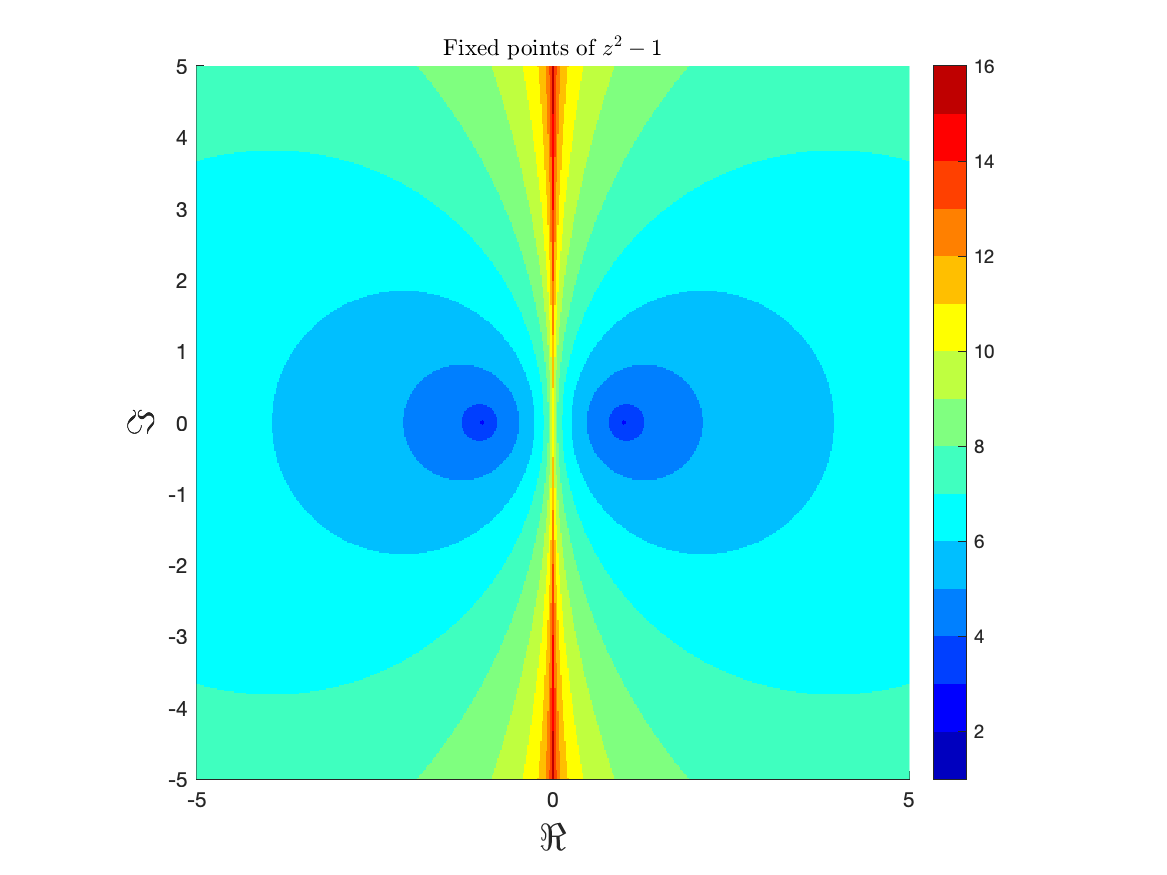
\includegraphics[width=\textwidth]{../Figures/Newton1.png}
		\caption{Iterations to roots of $z^2 - 1$}
		\label{fig:NI2}
	\end{subfigure}
	\begin{subfigure}[b]{\fwidth}
		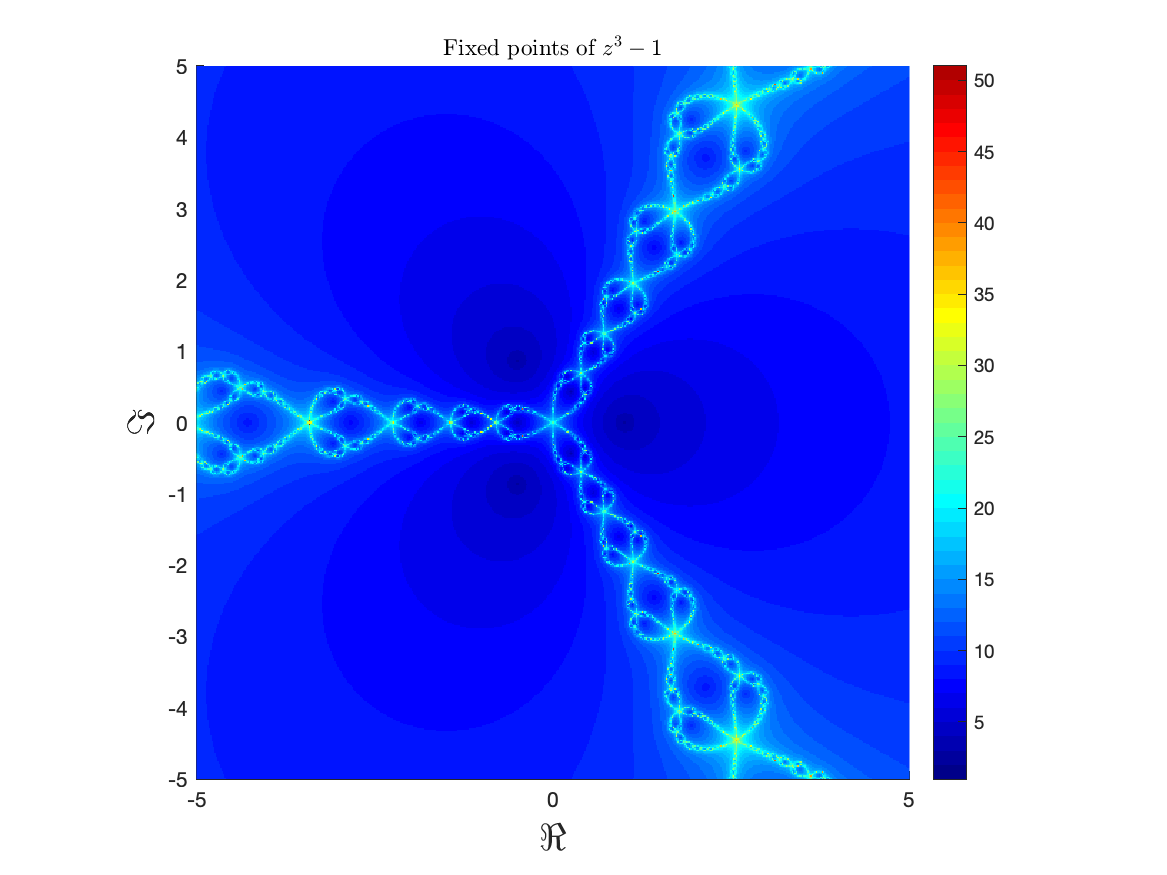
\includegraphics[width=\textwidth]{../Figures/Newton2.png}
		\caption{Iterations to roots of $z^3 - 1$}
		\label{fig:NI3}
	\end{subfigure}
	
	\vskip\baselineskip
	
	\begin{subfigure}[b]{\fwidth}
		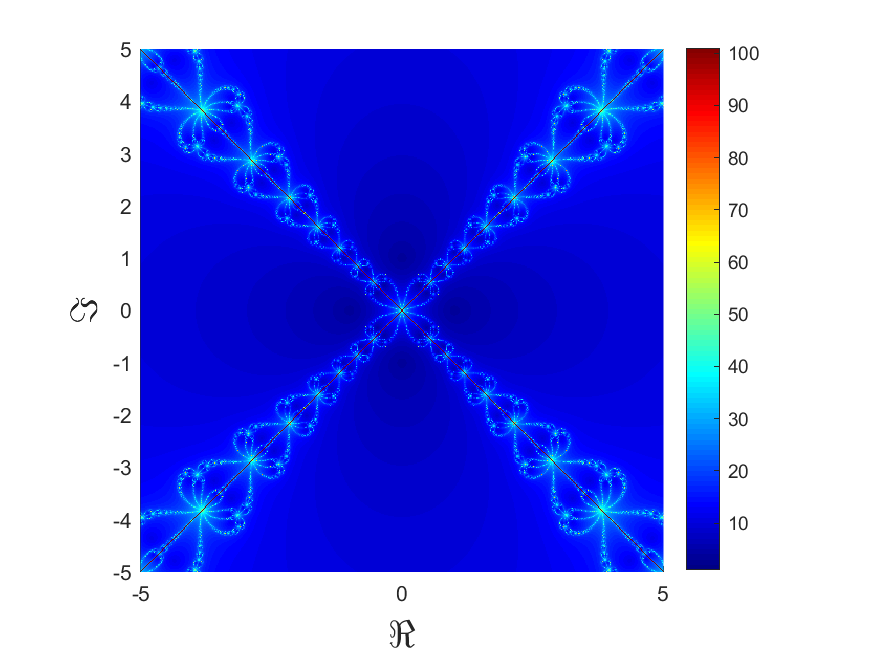
\includegraphics[width=\textwidth]{../Figures/Newton3.png}
		\caption{Iterations to roots of $z^4 - 1$}
		\label{fig:NI4}
	\end{subfigure}
	\begin{subfigure}[b]{\fwidth}
		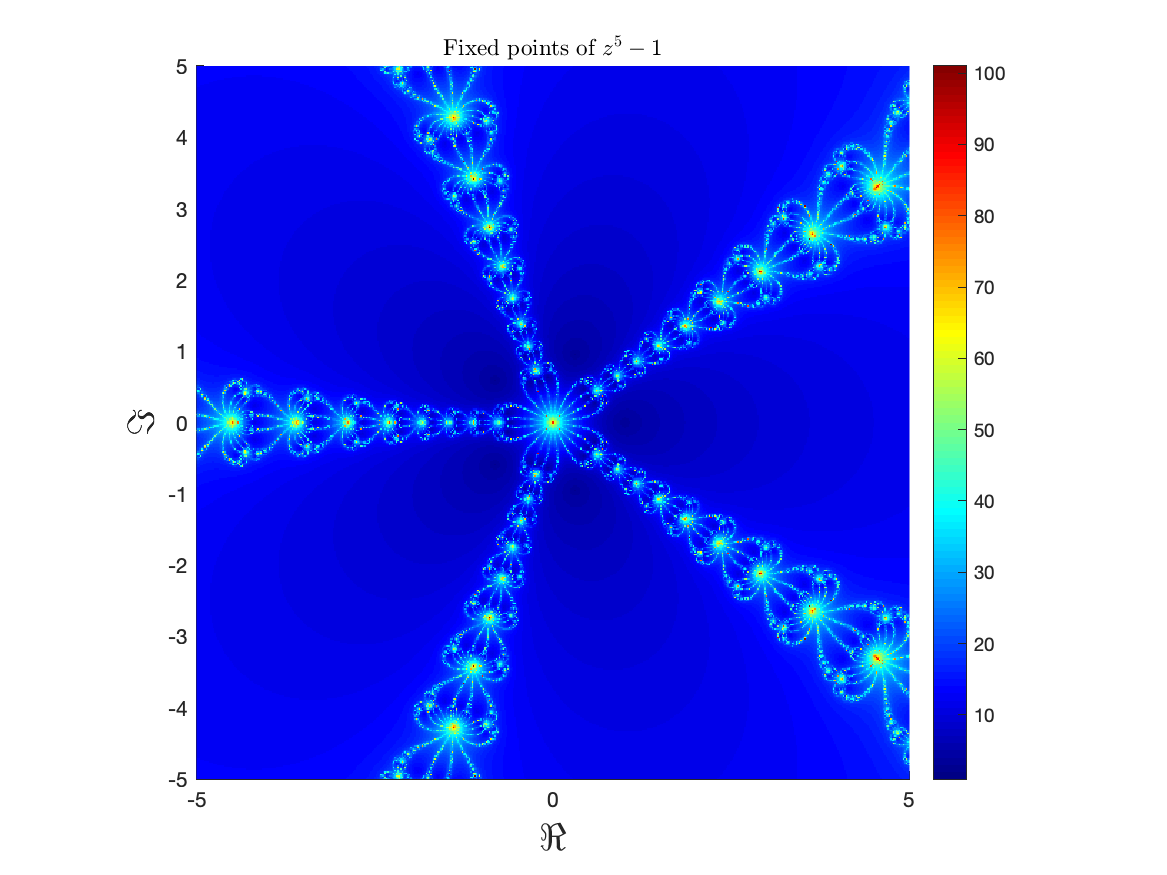
\includegraphics[width=\textwidth]{../Figures/Newton4.png}
		\caption{Iterations to roots of $z^5 - 1$}
		\label{fig:NI5}
	\end{subfigure}
	\caption{Roots of complex functions of form $z^n - 1$}
	\label{fig:NI}
\end{figure}

\section{The Mandelbrot Set}

\begin{figure}
	\centering
	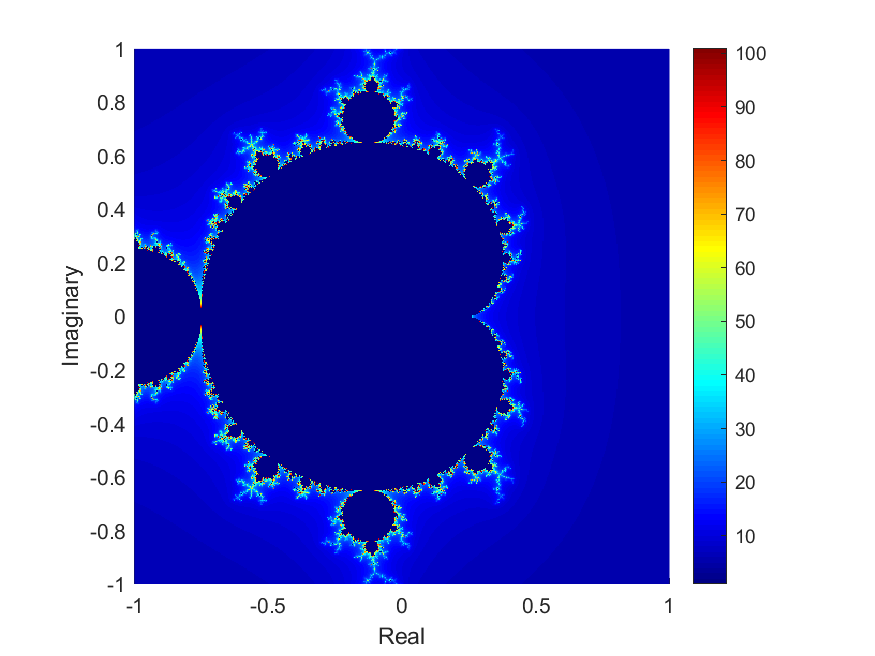
\includegraphics[width=3.5in]{../Figures/Mandelbrot.png}
	\caption{Mandelbrot set ...}
	\label{fig:Mandelbrot}
\end{figure}

\section{Conclusion}
Fractals are interesting shapes that come about when finding the orbits of complex functions. Due to the iterative nature of orbits, visually representing was a lengthy process. However, with computers, fractals can be easily visualized. One can switch the function under which the orbit is be calculated for with just a few keystrokes. Previously, this would have required manually recalculating the orbit of each of point. Fractals, which gets its name from fractional dimensions, are more than just interesting shapes. These fractals can represent important values for problem solving. Take Newton's iterations for example, the roots of an equation can be found by observing which values in the domain converge to a root the fastest. 

\newpage

\section{Appendix}

\subsection{Code}
\lstinputlisting[breaklines=true]{../Code/Project1.m}

\end{document}
